\begin{itemize}
	\item Let's think about the universal approximation theorem, proved by Hornik etal \cite{hornik1989multilayer}. A multilayer perceptron is a universal approximator of a function. Question though: can our problem be represented as a function? Let's think about a simple example of the input neurons being for $x$ and $y$ dimensions, and then the output being a singular neuron for $\cos(x)+\sin(y)$. That seems pretty sensible. I'm mostly concerned with how our input function is constructed so strangely. For example, if it's random whether $x$ or $y$ will be input to the first neuron, then this model breaks down.
	I do think the nature of the unreliability of this input vector means the approximation theorem doesn't apply. 
\end{itemize}

\section{FNN as a universal approximator}
There is a matter that cannot be ignored on this subject. The Universal Approximation Theorem for neural networks. Rigorously proved by Hornik, Stinchcombe, and White \cite{hornik1989multilayer}, the theorem's main points are:
\begin{itemize}
	\item Multilayer FNNs, even those with a single hidden layer, are universal approximators: they can approximate any continuous function to arbitrary accuracy.
	\item The above result is independent of choice of activation function so long as it is bounded and non-constant.
	\item Functions with finite support can be approximated exactly with a single hidden layer.
	\item Lack of success is due to insufficient number of hidden neurons \emph{or lack of a deterministic relationship between input and output}.
\end{itemize}
We emphasize the last point because it's believed this is the root cause of the failure of the FNN in learning the XTUD topologies. There is not consistency in what will appear in a given input node. For example, due to the randomness of the input loading, the same configuration may be loaded completely differently on separate instances.


\section{PCA detection of defects}
\subsection{Principal Component Analysis}
In this section we explore Principal Component Analysis (PCA) as a technique for detecting defect regions. PCA is a useful statistical method for transforming a dataset into a form that better distinguishes features in the data, and it may also be used as a dimension reduction tool on a dataset. It also falls into the category of unsupervised learning since it reveals features in the data without any label-directed goals. PCA is well-known, and we'll follow the explanation offered by Johnathan Shlens \cite{shlens2014pca}.

We let the $m\times n$ matrix $\bv{X}$ represent our dataset of $m$ observations on $n$ dimensions. The goal of PCA is to find the matrix $\bv{W}$ that \textit{best} transforms our dataset to a new set of orthogonal axes, or ``principal components'':
\begin{align*}
	\bv{Y} = \bv{X}\bv{W}.
\end{align*}
The $m\times n$ matrix $\bv{Y}$ then is our dataset projected onto this new set of axes. The \textit{best} axes of course are not arbitrary, but are such that they capture the maximal variance within the original dataset, with the variance monotonically decreasing with increasing axis index. In other words, the first PCA axis captures the largest variance, the second axis captures the next largest variance, and so on.
The column vectors $\bv{w_i}$ of $\bv{W}$ are in fact the unit vectors that describe the orientation of these new axes in the original $n$-dimensional space, and hence describe how each observation in $\bv{X}$ projects onto them.
The usefulness of this technique does rely on the assumption that a high variance along an axis indicates an important feature of the data, but this generally the case.

To begin, we note the covariance matrix of the $\bv{X}$ variables (adjusted to zero-mean to simplify calculations)
\begin{align*}
	\bv{C_X} = \frac{1}{m}\bv{X^TX}
\end{align*}
The diagonal elements of $\bv{C_X}$ are the variances of individual variables, and the off-diagonal elements are the covariances of different variables. We note that high covariances indicate a redundancy in our dataset, and we wish to minimize these.

We can now define a goal for optimizing $\bv{W}$: to diagonalize the covariance matrix $\bv{C_Y}$ of our transformed dataset. Such a matrix minimizes redundancy across variables and maximizes variance. There are multiple ways to diagonalize $\bv{C_Y}$, but PCA opts for a simple route by having PCA components form an orthonormal basis. 
To find $\bv{W}$ we perform an eigendecomposition on $\bv{C_Y}$ and find that the PCA components are in fact the eigenvectors of $\bv{C_X}$. We begin by writing $\bv{C_Y}$ in terms of $\bv{W}$:
\begin{align}
\nonumber	\bv{C_Y} &= \frac{1}{m}\bv{Y^TY}\\
\nonumber	&= \frac{1}{m}(\bv{W^TX^T})(\bv{XW})\\
\nonumber	&= \bv{W^T}\left(\frac{1}{m}\bv{X^TX}\right)\bv{W}\\
	&= \bv{W^TC_XW}.
\label{Eq:cycx}
\end{align}
We may draw on the property that any symmetric matrix $\bv{A}$ is diagonalizable, $\bv{A}=\bv{SDS^T}$, for diagonal eigenvalue matrix $\bv{D}$ and orthonormal eigenvector matrix $\bv{S}$. If we now define $\bv{W}$ as this matrix of eigenvectors for $\bv{C_X}$ (since $\bv{C_X}$ is symmetric), we have
\begin{align*}
	\bv{C_Y} &= \bv{W^T}(\bv{WDW^T})\bv{W}\\
	&= (\bv{W^TW})\bv{D}(\bv{W^TW})\\
	&= \bv{D},
\end{align*}
where we also use the orthonormality of $\bv{W}$. The eigenvalues, $\bv{\lambda}$, are also called the ``explained variance'' in this context. Their normalized values, $\lambda_i^* = \lambda_i/\sum\lambda_j$, or explained variance ratios, are used as a metric as to the importance of each axis, values close to $1$ indicate more significance and those closer to $0$ being less significant. Generally, one expects only some small number of dimensions to be significant and will see a noticeable drop in $\lambda^*$ indicating where component axes may be ignored.
We can verify that our conditions are met:
\begin{itemize}
	\item By Eq. \ref{Eq:cycx}, the $i$th diagonalized variance of $\bv{C_Y}$ is the variance of $\bv{X}$ along the $i$th principal component.
	\item $\bv{W}$ indeed diagonalizes $\bv{C_Y}$.
\end{itemize}

\subsection{PCA learning order parameters for phase transitions}
Recently, PCA has seen some fascinating use on condensed matter systems. In 2016, L.\ Wang (Ref.\ \cite{wang2016ising}), with a dataset of simulated Ising spin systems (each observation was an instance of a system and each spin location was a feature dimension of $\bv{X}$), PCA could locate phase transitions in both the standard Ising model, but also the conserved order parameter (COP) Ising model. In the standard model, reduction showed that only the first PCA component was significant for capturing the distinguishing information of the system. Indeed, the corresponding eigenvector $\bv{w_1}$ was simply a constant function, meaning that it was in fact the magnetization order parameter, and cluster analysis of the data along this component (although it was also visually evident) showed two clusters corresponding to the high and low temperature states. The author took things a step further with the COP model because each system had a net-zero magnetization, so the magnetization order parameter would not suffice and PCA would need to find other indicators of the phase transition. Championing this restriction, PCA found that four components were all that was necessary and together could form the structure factor indicative of the phase transition.

In 2018, authors R.B.\ Jadrich \textit{et al.}\ (Ref.\ \cite{jadrich2018offlattice}) applied PCA to detect phase transitions of multiple off-lattice systems, including the fluid-nematic transition of a liquid crystal system much like the one of focus here (although with ellipsoid molecules as opposed to rod-like). Their methods were similar to those just described, but instead of each observation being a whole system, they were smaller local samples centered on random probe molecules (e.g.\ the orientations of 20 nearest neighbours). Additionally, the off-lattice nature carried with it some ambiguity as to the structuring/ordering of the nearest neighbours that formed $\bv{X}$ dimensions. Using an intuitive distance-to-probe ordering, they found again only the first PCA component was needed to learn the transition, and that it modeled the classical order parameter used to locate the transition.

What is crucial to note here, and what is so exceptional about this method, is that, apart from the raw particle information (location, spin, orientation, etc.), it requires no additional information about each system such as Hamiltonians or interaction potentials. On top of this, PCA does not cluster observations in some black-box style, but discovers the precise order parameters that are classically used to indicate the phase change.

\subsection{PCA learning disclinations}
We now put forth the question: Can PCA use nearest neighbour information of our LC system to identify nematic vs.\ disclination/defect states of the variety shown in Fig, or beyond that which \textit{type} of defect?
The following discusses this question, with results on the endeavor presented in Sec.\ \ref{Results}.

The results of Ref.\ \cite{jadrich2018offlattice} are certainly encouraging, though their objective was somewhat different. PCA detected a long-range angular correlation appeared signaling the nematic phase, and for this they used every \nth{10} nearest neighbour. Here we are concerned with detailed local features. In theory, the nematic vs.\ non-nematic states should be differentiable. For a given probe $i$ (either a rod or a point in space), we may construct a feature vector $f_i = [x_1^{(i)},x_2^{(i)},\cdots,x_{nn}^{(i)}]$ of some physical quantity $x$. Rod orientation relative to the probe rod $\theta_{ij}$ or, to account for the rod symmetry, the transformed $\cos(2\theta_{ij})$ may be sufficient, but the probe rod orientation is highly variable within a characteristic defect orientation, so defects may appear significantly different in their feature vectors. A counter to this would to take neighbouring rod orientations with respect to a local nematic director $\alpha$ isntead. 

A random ordering of neighbours may work in detecting nematic vs.\ defect states, but would not be expected to work for the more detailed defect type detection. In a perfectly shaped defect, a maximal $\theta_{\alpha j}$ or frequency of certain angles may signal a defect type, but the Monte Carlo defect samples would have too much overlap/similarity for a randomly ordered feature vector. Thus, in the same way that humans visually identify winding numbers, a feature vector that is ordered by a clockwise procession around the defect center should be a more effective approach.



\begin{figure*}[!t]
	\centering
	\begin{minipage}[t]{0.25\textwidth}
		\centering
		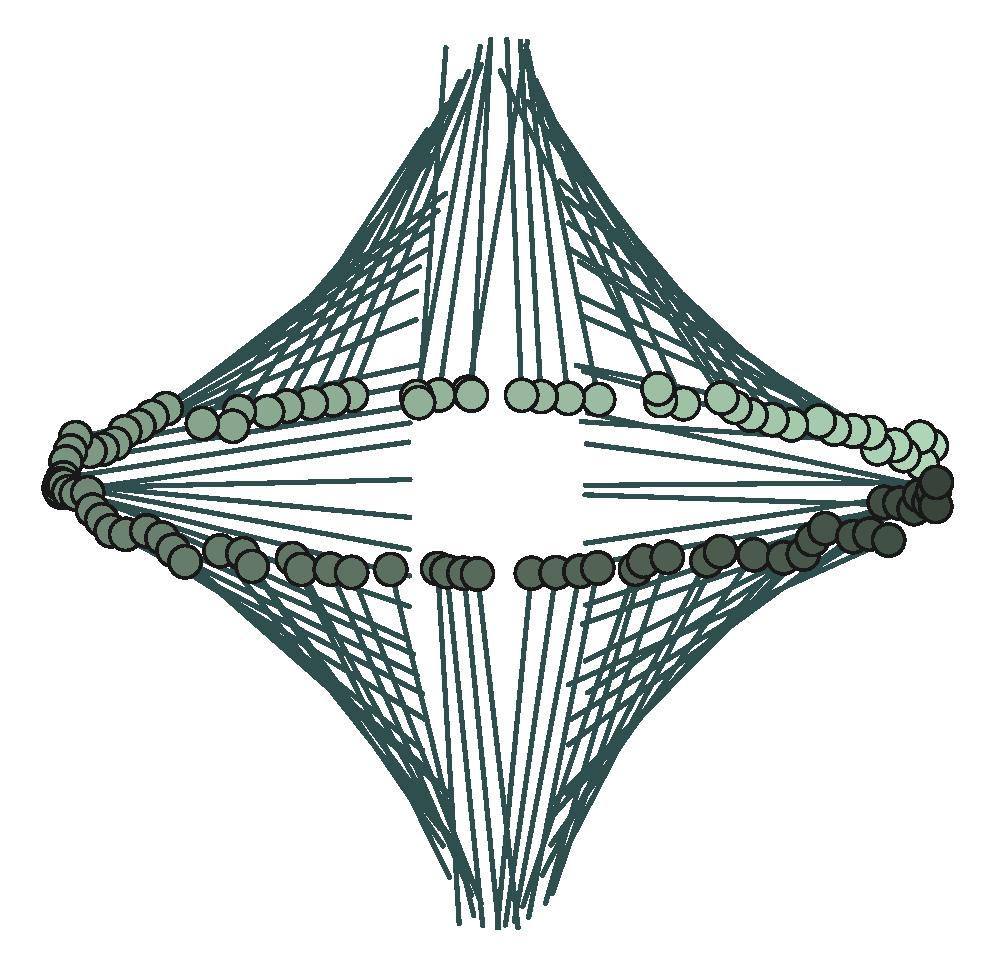
\includegraphics[width=0.9\columnwidth]{./figs/minusone_reruns_0_alt.eps}\\
		(a)\\ \vspace{0.5cm}
		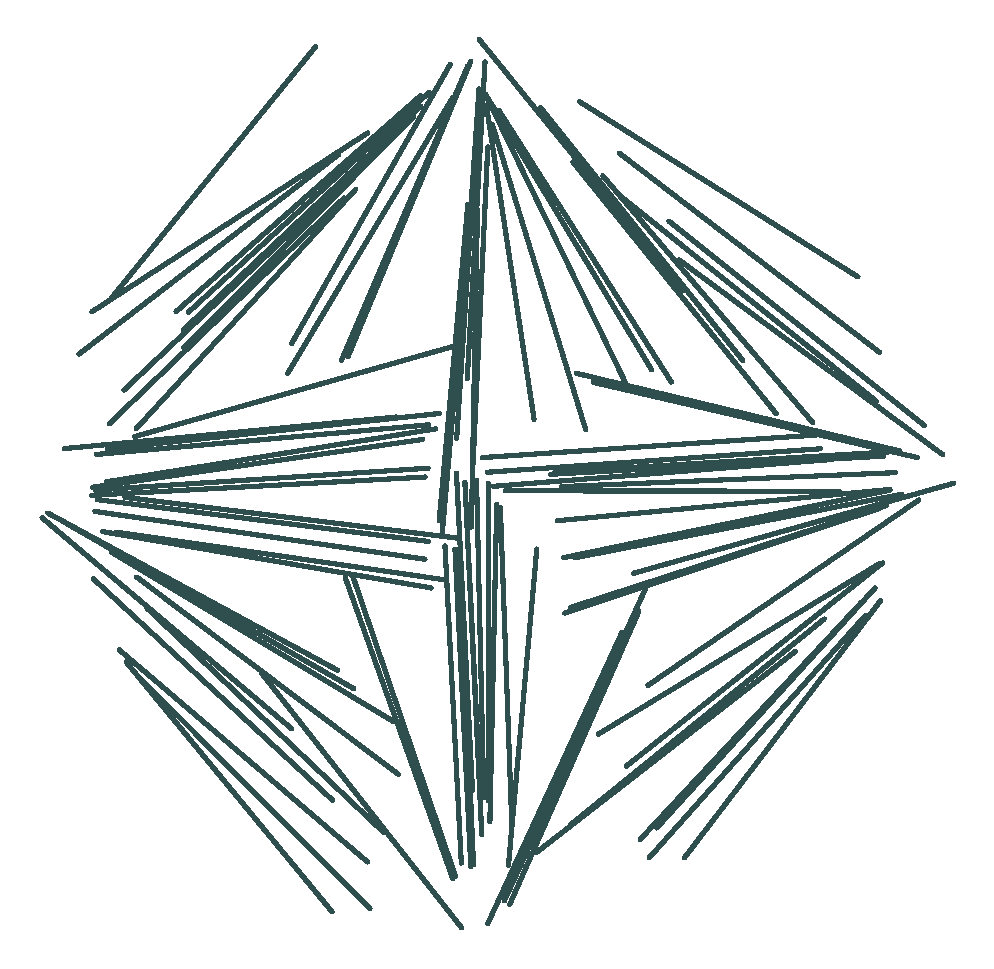
\includegraphics[width=0.9\columnwidth]{./figs/minusone_reruns_1_alt.eps}\\
		(e)
	\end{minipage}%
	\begin{minipage}[t]{0.25\textwidth}
		\centering
		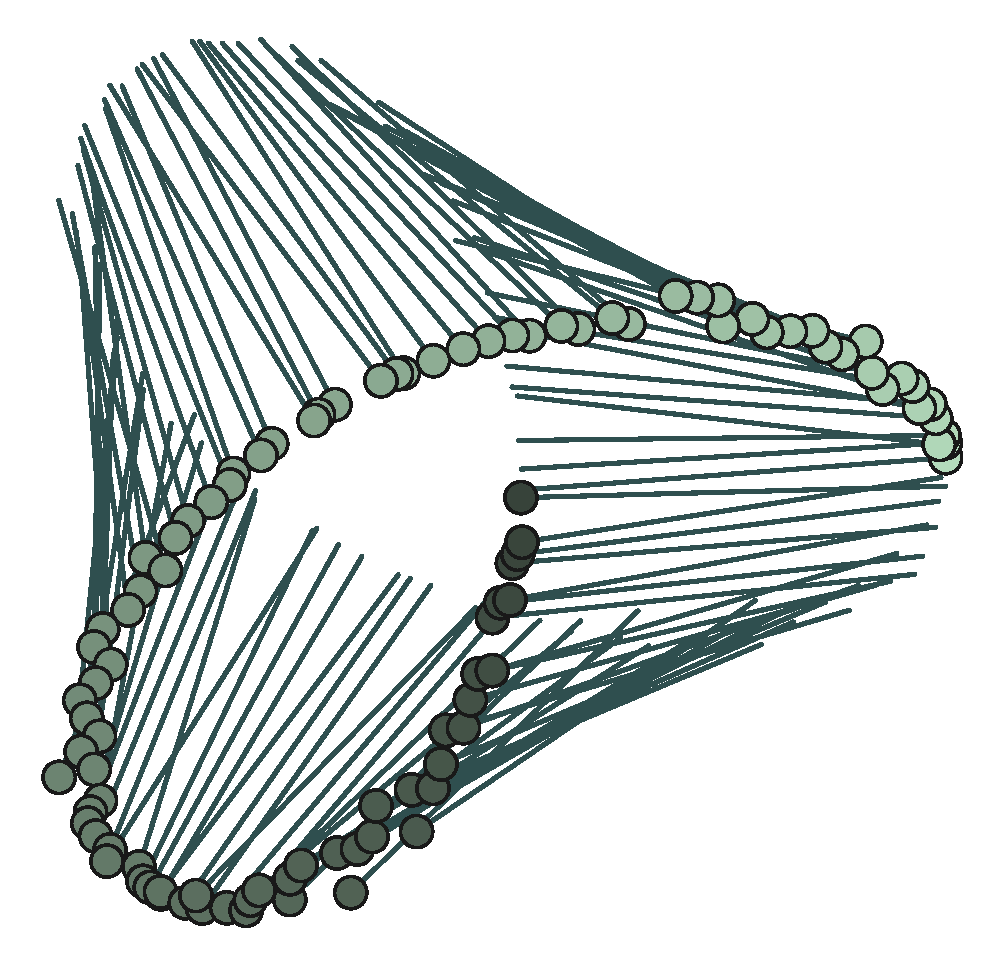
\includegraphics[width=0.9\columnwidth]{./figs/minushalf_reruns_0.eps}\\
		(b)\\ \vspace{0.5cm}
		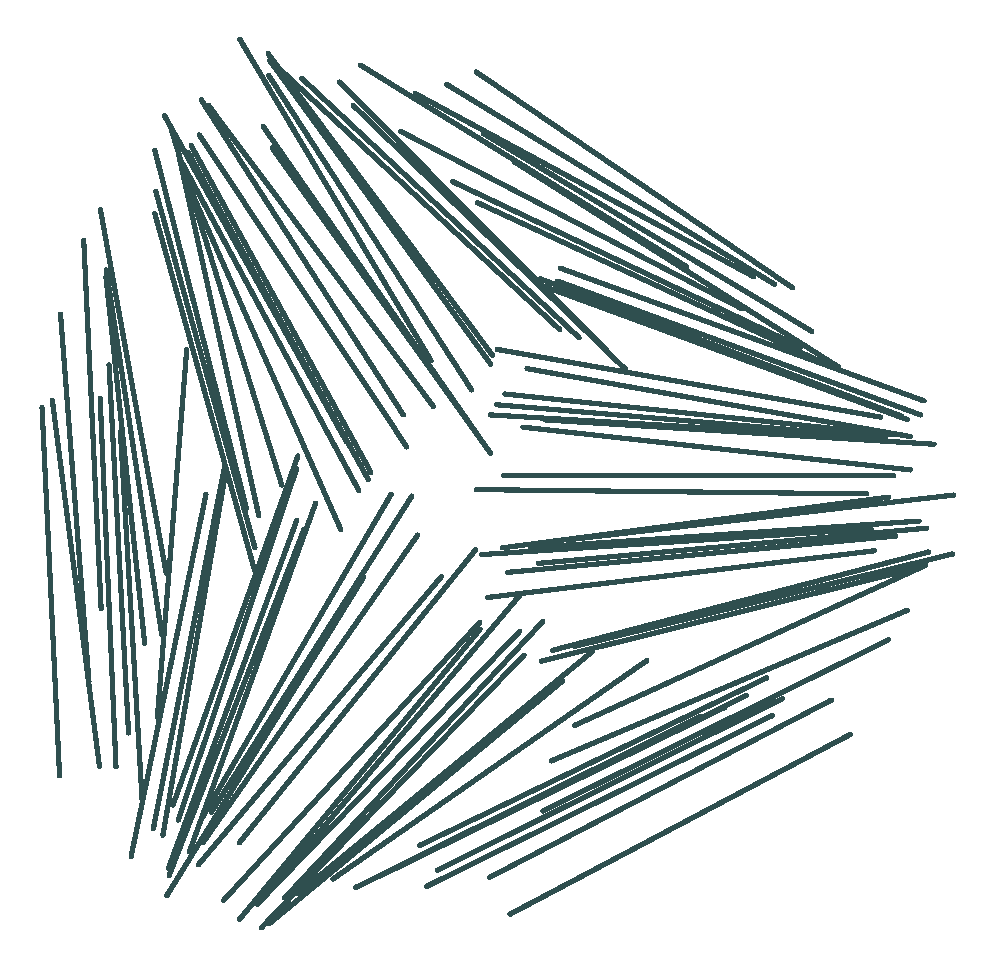
\includegraphics[width=0.9\columnwidth]{./figs/minushalf_reruns_1.eps}\\
		(f)
	\end{minipage}%
	\begin{minipage}[t]{0.25\textwidth}
		\centering
		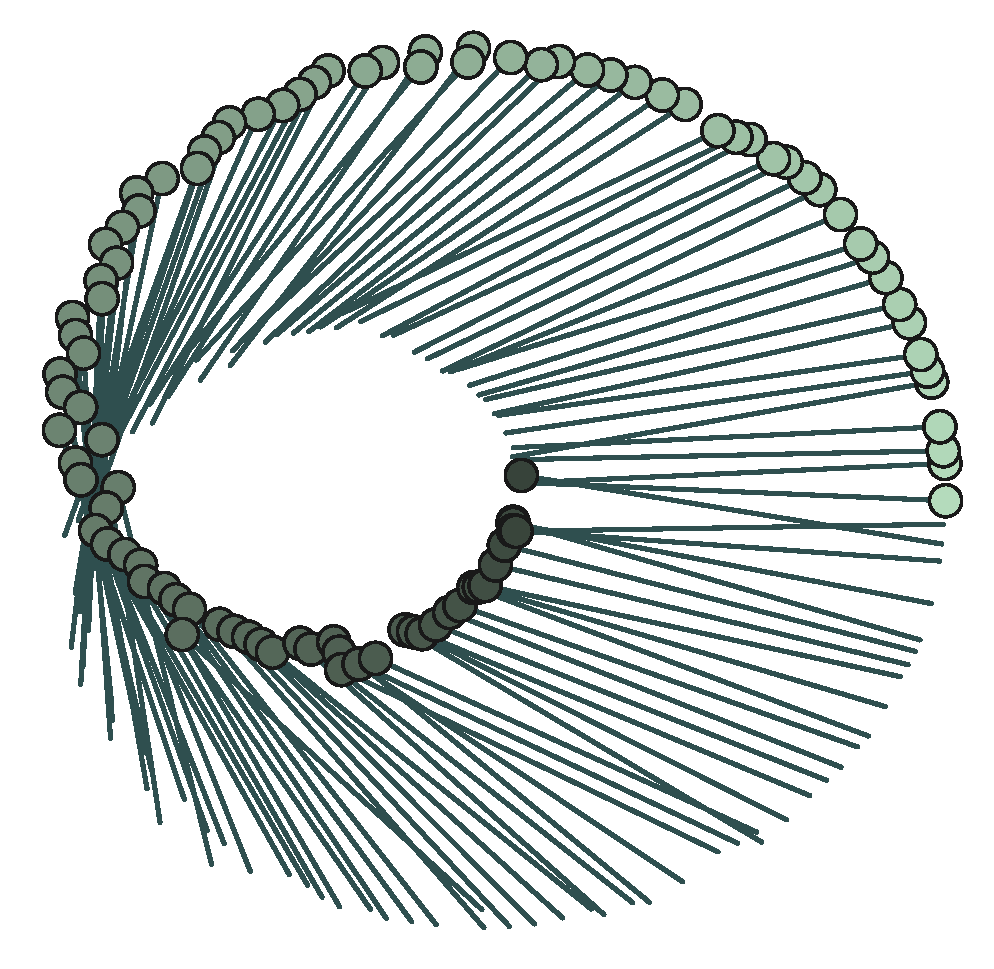
\includegraphics[width=0.9\columnwidth]{./figs/plushalf_reruns_0.eps}\\
		(c)\\ \vspace{0.5cm}
		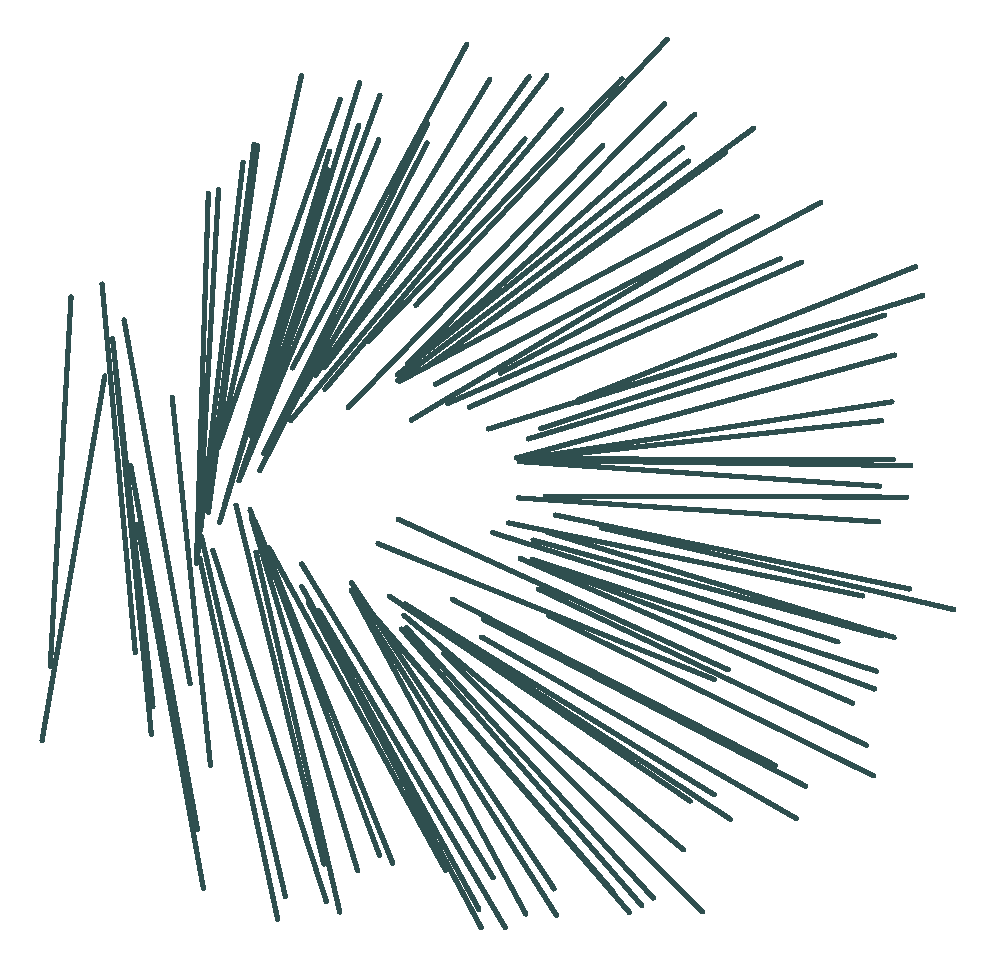
\includegraphics[width=0.9\columnwidth]{./figs/plushalf_reruns_1.eps}\\
		(g)
	\end{minipage}%
	\begin{minipage}[t]{0.25\textwidth}
		\centering
		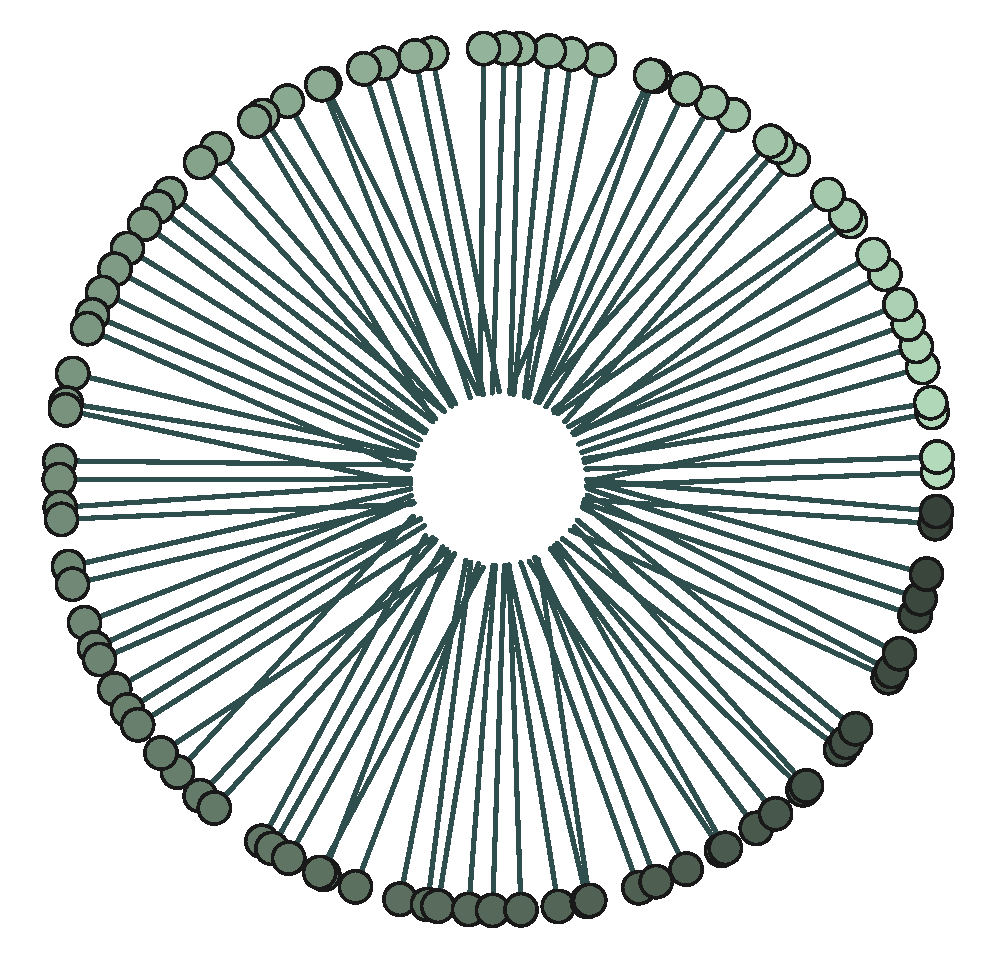
\includegraphics[width=0.9\columnwidth]{./figs/plusone_reruns_0.eps}\\
		(d)\\ \vspace{0.5cm}
		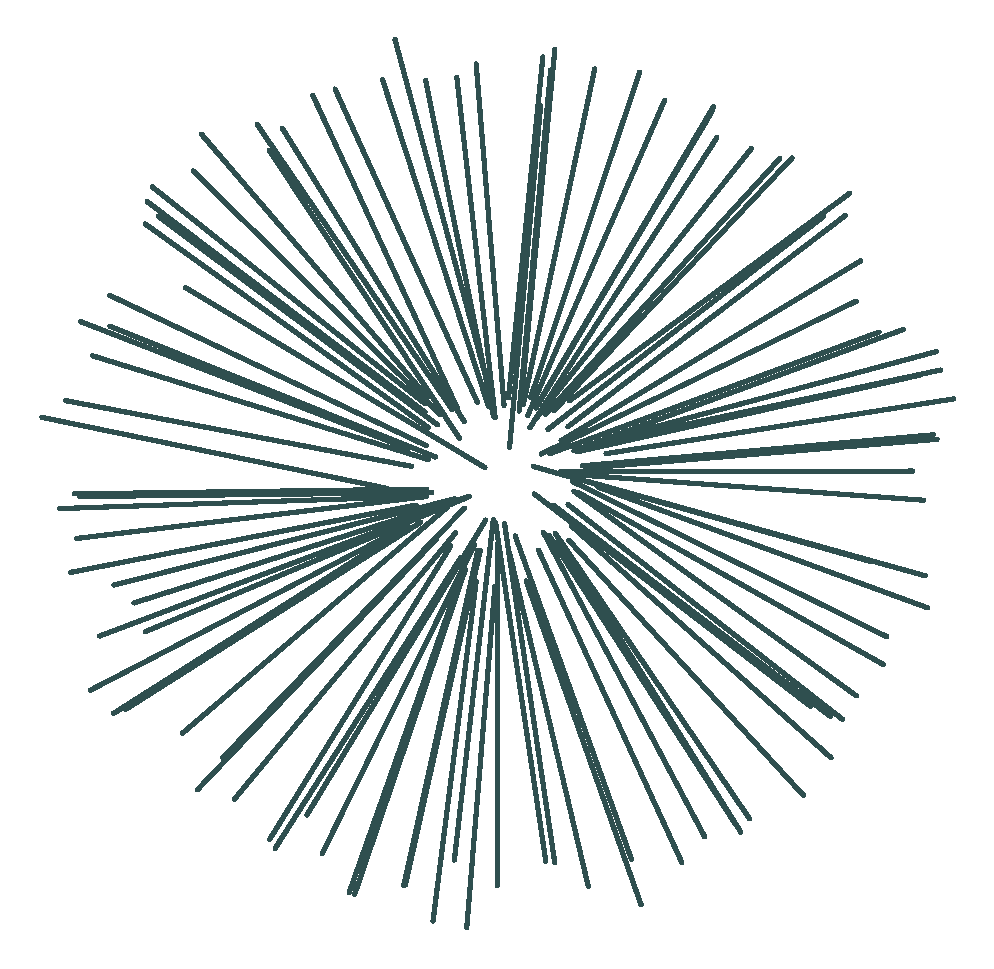
\includegraphics[width=0.9\columnwidth]{./figs/plusone_reruns_1.eps}\\
		(h)
	\end{minipage}%
	\caption{(a)-(d) Examples of initialized disclinations with winding numbers $-1$, $-1/2$, $+1/2$, and $+1$ respectively, as a visual aid for understanding the procession around the defect center. In proceeding clockwise around a defect, winding polarity indicates the direction of rotation about the rod axis, and magnitude indicates how many rotations about this axis. Coloured dots are included as a visual aid. (e)-(h) Below, uncrossed samples of the above disclinations. Such uncrossed samples made up the defect PCA dataset.
	}
	\label{FIG:defects_pure}
\end{figure*}

We adopt an approach where we first identify a nematic director $\alpha$ from neighbours. We use a discretized version of the method outlined in Section \ref{Order param} that produces the $Q$-matrix in equation \ref{eq:Qmat}:
\begin{align*}
	Q_{nn} = \frac{1}{2}\left(
	\begin{matrix}
	S_{nn}(x,y) & T_{nn}(x,y)\\
	T_{nn}(x,y) & -S_{nn}(x,y).
	\end{matrix}
	\right)
\end{align*}
where $S_{nn}$ and $T_{nn}$ are averaged over neighbours,
\begin{align*}
	S_{nn} &= \frac{1}{N_{nn}}\sum_i \cos(2\theta_i)\\
	T_{nn} &= \frac{1}{N_{nn}}\sum_i \sin(2\theta_i)
\end{align*} 











